%%%%%%%%%%%%%%%%%%%%%%%%%%%%%%%%%%%%%%%%%
% Dreuw & Deselaer's Poster
% LaTeX Template
% Version 2.0 (February 18, 2023)
%
% This template originates from:
% https://www.LaTeXTemplates.com
%
% Authors:
% Vel (vel@latextemplates.com)
% Philippe Dreuw and Thomas Deselaers (https://github.com/deselaers/latex-beamerposter)
%
% License:
% CC BY-NC-SA 4.0 (https://creativecommons.org/licenses/by-nc-sa/4.0/)
%
% NOTE: The bibliography needs to be compiled using the bibtex engine.
%
%%%%%%%%%%%%%%%%%%%%%%%%%%%%%%%%%%%%%%%%%

%----------------------------------------------------------------------------------------
%	PACKAGES AND OTHER DOCUMENT CONFIGURATIONS
%----------------------------------------------------------------------------------------

\documentclass{beamer} % Use the beamer base class

\usepackage[
	orientation=portrait, % Portrait orientation
	size=a0, % Paper size
	scale=1.21, % Scale, it's important to adjust this so your content fits nicely in the template
]{beamerposter} % Use the beamerposter package to create the layout

\usetheme{I6pd2} % Use the I6pd2 theme supplied with this template

\def\E{\mathbb{E}} % Expectation symbol
\newcommand{\x}{\textbf{v}}

\usepackage{changepage} % Required for temporarily indenting text blocks

\usepackage{amsmath,amsthm,amssymb,latexsym} % For including math equations, theorems, symbols, etc

\usepackage{gfsdidot} % Use the GFS Didot font

\usepackage{booktabs} % Top and bottom rules for tables

\graphicspath{{Figures/}} % Location of figure images

%----------------------------------------------------------------------------------------
%	TITLE SECTION
%----------------------------------------------------------------------------------------

\title{\LARGE Volatility Forecasting Using Similarity-based Parameter Correction and Aggregated Shock Information} % Poster title

\author{David P. Lundquist\textsuperscript{1} and Daniel J. Eck\textsuperscript{1}} % Author(s)

\institute{\textsuperscript{1}Department of Statistics, University of Illinois Urbana-Champaign} % Institution(s)

%----------------------------------------------------------------------------------------
%	FOOTER TEXT
%----------------------------------------------------------------------------------------

\newcommand{\leftfoot}{https://www.LaTeXTemplates.com} % Left footer text

\newcommand{\rightfoot}{john@latextemplates.com} % Right footer text

\setbeamertemplate{footline}{} % Uncomment this line to hide the footer

%----------------------------------------------------------------------------------------

\begin{document}

\begin{frame}[t] % The whole poster is enclosed in one beamer frame, the [t] parameter aligns everything to the top

\begin{columns}[t] % Begin multi-column layout, the [t] parameter aligns each column's content to the top

\begin{column}{0.02\textwidth}\end{column} % Empty column for horizontal whitespace

\begin{column}{0.465\textwidth} % Start the first content column

%----------------------------------------------------------------------------------------
%	OBJECTIVES
%----------------------------------------------------------------------------------------

\begin{block}{Introduction}
	\begin{enumerate}
		\item Reacting to a seemingly unprecedented event might involve the question: what, if anything, does it resemble from the past?  
		\item Matching a current crisis to past events is a problem with unsurprising statistical angles: identification, sample size, weighting, risk, and robustness.
		\item Here we employ a method to improve our GARCH volatility forecasts under unprecedented conditions.
	\end{enumerate}
\end{block}

%----------------------------------------------------------------------------------------
%	INTRODUCTION
%----------------------------------------------------------------------------------------
            
\begin{block}{Setting}
	Donec fringilla
	\bigskip % Vertical whitespace


		$\sigma_{t}^{2} = \omega+ \sum^{m}_{k=1}\alpha_{k}a^{2}_{t-k} + \sum_{j=1}^{s}\beta_{j}\sigma_{t-j}^{2} + \gamma^{T}\x_{t} \text{ .}\label{GARCH-X}$

	\end{block}

%----------------------------------------------------------------------------------------
%	MATERIALS
%----------------------------------------------------------------------------------------

\begin{block}{Methodology}


	\begin{itemize}

		\item Vestibulum nisl, quis euismod velit eros in ligula.
		\begin{itemize}
			\item Cras rhoncus quam et augue convallis in elementum urna tincidunt.
		\end{itemize}
		\item Proin ut vestibulum augue.
		\begin{itemize}
			\item Donec dapibus sagittis neque eu ultrices.
		\end{itemize}

	\end{itemize}

	
		% $\text{Forecast 1: } & \hat\sigma^{2}_{unadjusted} = \hat\E[\sigma^{2}_{1,T_{1}^{*}+1}|\mathcal{F}_{T^{*}}] = \hat\omega_{i} + \sum^{m_{i}}_{k=1}\hat\alpha_{i,k}a^{2}_{i,t-k} + \sum_{j=1}^{s_{i}}\hat\beta_{i,j}\sigma_{i,t-j}^{2} + \hat\gamma_{i}^{T} \x_{i,t}\\
		% \text{Forecast 2: } & \hat\sigma^{2}_{adjusted} = \hat\E[\sigma^{2}_{1,T_{1}^{*}+1}|\mathcal{F}_{T^{*}}] + \hat\omega^{*} = \hat\omega_{i} + \sum^{m_{i}}_{k=1}\hat\alpha_{i,k}a^{2}_{i,t-k} + \sum_{j=1}^{s_{i}}\hat\beta_{i,j}\sigma_{i,t-j}^{2} + \hat\gamma_{i}^{T} \x_{i,t} + \hat\omega^{*} \text{ .}$

	
	\bigskip % Vertical whitespace
	
\end{block}

%----------------------------------------------------------------------------------------
%	METHODS
%----------------------------------------------------------------------------------------

\begin{block}{Loss Functions}	
	\begin{itemize}
		\item International support:
		\begin{itemize}
			\item àáâäãåèéêëìíîïòóôöõøùúûüÿýñçčšž
			\item ÀÁÂÄÃÅÈÉÊËÌÍÎÏÒÓÔÖÕØÙÚÛÜŸÝÑ
			\item ßÇŒÆČŠŽ
		\end{itemize}
		\item Maecenas Vel Nisl Elit
		\begin{itemize}
			\item Suspendisse potenti. Fusce a est eget turpis rhoncus varius sed sed dui. Cras justo nibh, bibendum a cursus eget, consequat et dui. Maecenas vel nisl elit, sed dignissim dolor. 
			\item In hac habitasse platea dictumst.
		\end{itemize}
		
		\item Viewpoint Matching Constraints
		\begin{itemize}
			\item Cum sociis natoque penatibus et magnis dis parturient montes, nascetur ridiculus mus. 
			\item Proin in nisi diam.
			\item Nam ultricies pellentesque nunc, ultrices volutpat nisl ultrices a.
		\end{itemize}
	\end{itemize}
\end{block}

%----------------------------------------------------------------------------------------
%	MATHEMATICS
%----------------------------------------------------------------------------------------

\begin{block}{Properties of Volatility Shocks and Shock Estimators}

	% \begin{prop}\label{omega_consistency}
	% 	Assume
	% 	\begin{enumerate}
	% 	  \item For each $i$, $\{a_{i,t}\}_{t=0,...,T_i}$ obeys a GARCH-X($m,s$), as laid out in Equation $\eqref{GARCH-X}$, with volatility shocks found in $\mc{M}_{1}$, where $T_i$ is the length of the $i$th series.
	% 	  \item For each $i, \{\omega_{i,t}^{*}\}_{t=0,...,T_i}$ is potentially non-zero at $\{T^{*}_{i}+1,... ,T^{*}_{i}+k\}$, $\omega_{i,T^{*}+1}^{*}\equiv...\equiv\omega_{i,T^{*}+k}^{*}$, and zero otherwise, where the arrival of $T_{i}^{*}$ is governed by a time-invariant distribution on $\{a_{i,t}\}_{t=0,...,T_i-1}$. \label{stationarity_of_omega_i_t}
	% 	  \item The conditions in Assumption 0 of \citet{han2014asymptotic} prevail.
	% 	\end{enumerate}
	% 	Then for any $i$, $\hat\omega_{i,t}^{*} \xlongrightarrow{p} \omega_{i,T^{*}+1}^{*}$ as $t\rightarrow\infty$.
	% 	\end{prop}
\end{block}

%----------------------------------------------------------------------------------------

\end{column} % End of the first column

\begin{column}{0.03\textwidth}\end{column} % Empty column for horizontal whitespace
 
\begin{column}{0.465\textwidth} % Start the second content column

%----------------------------------------------------------------------------------------
%	RESULTS
%----------------------------------------------------------------------------------------

\begin{block}{Numerical Examples}
	\begin{itemize}
		\item Ased Aliquet Luctus Lectus
	\end{itemize}
	
	\begin{table}
		\caption{Table caption.}
		\begin{tabular}{l l l}
			\toprule
			\textbf{Treatments} & \textbf{Response 1} & \textbf{Response 2}\\
			\midrule
			Treatment 1 & 0.0003262 & 0.562 \\
			Treatment 2 & 0.0015681 & 0.910 \\
			Treatment 3 & 0.0009271 & 0.296 \\
			\bottomrule
		\end{tabular}
	\end{table}
	
	\bigskip\bigskip % Vertical whitespace
	
	Aliquam arcu turpis, ultrices sed luctus ac, vehicula id metus. Morbi eu feugiat velit, et tempus augue. Proin ac mattis tortor. Donec tincidunt, ante rhoncus luctus semper, arcu lorem lobortis justo, nec convallis ante quam quis lectus.
	
	\begin{table} % Single column table
		\caption{Another table caption.}
		\begin{tabular}{l l r}
			\toprule
			\multicolumn{2}{c}{\textbf{Location}} \\
			\cmidrule(r){1-2}
			East Distance & West Distance & Count \\
			\midrule
			100km & 200km & 422 \\
			350km & 1000km & 1833 \\
			600km & 1200km & 890 \\
			\bottomrule
		\end{tabular}
	\end{table}
	
	\bigskip\bigskip % Vertical whitespace
	
	\begin{itemize}
		\item Vivamus lobortis eros et massa porta porttitor.
	\end{itemize}
\end{block}

%------------------------------------------------

\begin{block}{Real Data Example: Aftermath of Donald Trump's 2016 Victory}
	\begin{figure}
		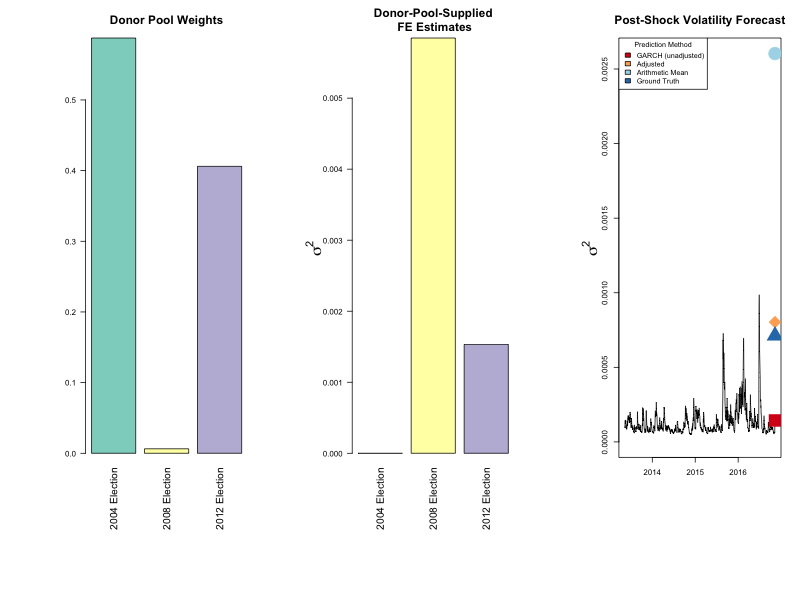
\includegraphics[width=\linewidth]{../real_data_output_plots/FriMay311830522024_IYG_None_2016-06-22.png}
		\caption{Bovine pulmonary artery endothelial cells in culture. Blue: nuclei; red: mitochondria; green: microfilaments. Computer generated image from a 3D model based on a confocal laser scanning microscopy using fluorescent marker dyes.}
	\end{figure}
\end{block}

%----------------------------------------------------------------------------------------
%	CONCLUSIONS
%----------------------------------------------------------------------------------------

\begin{block}{Conclusions}
	\begin{enumerate}
		\item \alert{Opet volutpat ligula.} Duis semper lorem eget dui dignissim porttitor. Nulla facilisi. In ullamcorper lorem quis dolor iaculis nec egestas enim ultricies. Cras ut mauris elit, ut lacinia dui. Proin in ante et libero hendrerit iaculis.
	\end{enumerate}
\end{block}

%----------------------------------------------------------------------------------------
%	REFERENCES
%----------------------------------------------------------------------------------------

\begin{block}{References}
	\nocite{*} % Insert publications even if they are not cited in the poster
	\small % Reduce font size
	\vspace{-1ex} % Pull up slightly
	\bibliographystyle{unsrt} % Bibliography style
	\bibliography{../synthVolForecast.bib} % Bibliography file
\end{block}

%----------------------------------------------------------------------------------------
%	ACKNOWLEDGEMENTS
%----------------------------------------------------------------------------------------

\begin{block}{Acknowledgements}
	\textbf{Nam mollis} tristique neque eu luctus. Suspendisse rutrum congue nisi sed convallis. Aenean id neque dolor. \textbf{Pellentesque habitant} morbi tristique senectus et netus et malesuada fames ac turpis egestas.
\end{block}

%----------------------------------------------------------------------------------------
%	CONTACT INFORMATION
%----------------------------------------------------------------------------------------

\setbeamercolor{block title}{fg=black, bg=taorange} % Change the block title color

\begin{block}{Contact Information}
	\begin{itemize}
		\item Web: \href{https://www.university.edu/labname}{https://www.university.edu/labname}
		\item Email: \href{mailto:davidl11@illinois.edu}{davidl11@illinois.edu}
	\end{itemize}
\end{block}

%----------------------------------------------------------------------------------------

\end{column} % End of the second column

\begin{column}{0.02\textwidth}\end{column} % Empty column for horizontal whitespace

\end{columns} % End of all the columns in the poster

\end{frame} % End of the enclosing frame

%----------------------------------------------------------------------------------------

\end{document}
